\documentclass{article}
\usepackage{hyperref}
\usepackage{graphicx}
\begin{document}
\title{Measuring Icebergs: Different Estimates of COVID-19 Cases in Portugal}
\author{$@$CoronaSurveys Team \\ \texttt{https://github.com/GCGImdea/coronasurveys}}
\maketitle
\section{Introduction}

During the current coronavirus pandemics, monitoring the evolution of COVID-19 cases is an important component for awareness and to inform policy decisions. 
Official numbers of laboratory confirmed cases are periodically issued by each country's health authority, for Portugal see \url{https://covid19.min-saude.pt}. 

Typically, along an outbreak testing eligibility criteria can evolve and the number of available tests also. Under these circumstances the evolution of official laboratory confirmed cases might not represent the total number of cases (see \url{https://www.nature.com/articles/d41586-020-00760-8}).  

This motivates looking at other probing techniques and try to bring in more information about the potential numbers. Actually the true numbers might only be known in the future once serological surveys are done (as done in prior outbreaks \url{https://journals.plos.org/plosone/article?id=10.1371/journal.pone.0050770}.

Bellow we consider two approaches: (a) Inferring current cases from the case fatality series; (b) Using crowdsourcing with anonymous surveys of indirect information.  

\section{Delay-adjusted case fatality ratio}

If we look at the current number of fatalities and divide it with the current number of confirmed cases, we obtain a naive case fatality ratio (CFR). However this metric does not take into account the number of cases with known outcomes, since recent cases will still evolve into fatalities and recoveries. By estimating the true number of cases with known outcomes, it is possible to obtain a corrected case fatality ratio (cCFR), as in \url{https://journals.plos.org/plosone/article?id=10.1371/journal.pone.0006852}, that takes into account the average delay from symptoms to death.  

Since the corrected denominator (cases with known outcomes) is reduced, the cCFR is higher than the naive CFR during a growing outbreak. A high cCFR is typically an indicator of lack of coverage in laboratory testing. If we assume, in general, that the disease will have similar case fatality rates in different countries it is possible use the known fatality ratio from Wuhan, China, currently at $1.38\%$
to compare with the obtained cCFR and estimate the percentage of coverage in different countries. This is done in \url{https://cmmid.github.io/topics/covid19/severity/global_cfr_estimates.html} and, for instance, the projected coverage in Portugal and Spain is $19\%$ and $4.7\%$. These values can in turn be used to correct the number of reported confirmed cases in each country an estimate the likely true number of cases, thus probing the iceberg that lurks under water.

Another technique, based on the same corrections, but using an overall gross value for estimating the true cases from the mortality rate is simply obtained by multiplying the cumulative mortality by 400. See \url{https://www.nature.com/articles/d41586-020-00760-8}. We will use both techniques for estimation in each country.

\section{Crowdsourcing with anonymous surveys}

\section{The Portuguese data}

Portuguese data on fatality and confirmed cases was obtained in \url{https://github.com/dssg-pt/covid19pt-data}, a public repository that helps disseminated the official DGS daily data.

\begin{figure}
\begin{center}
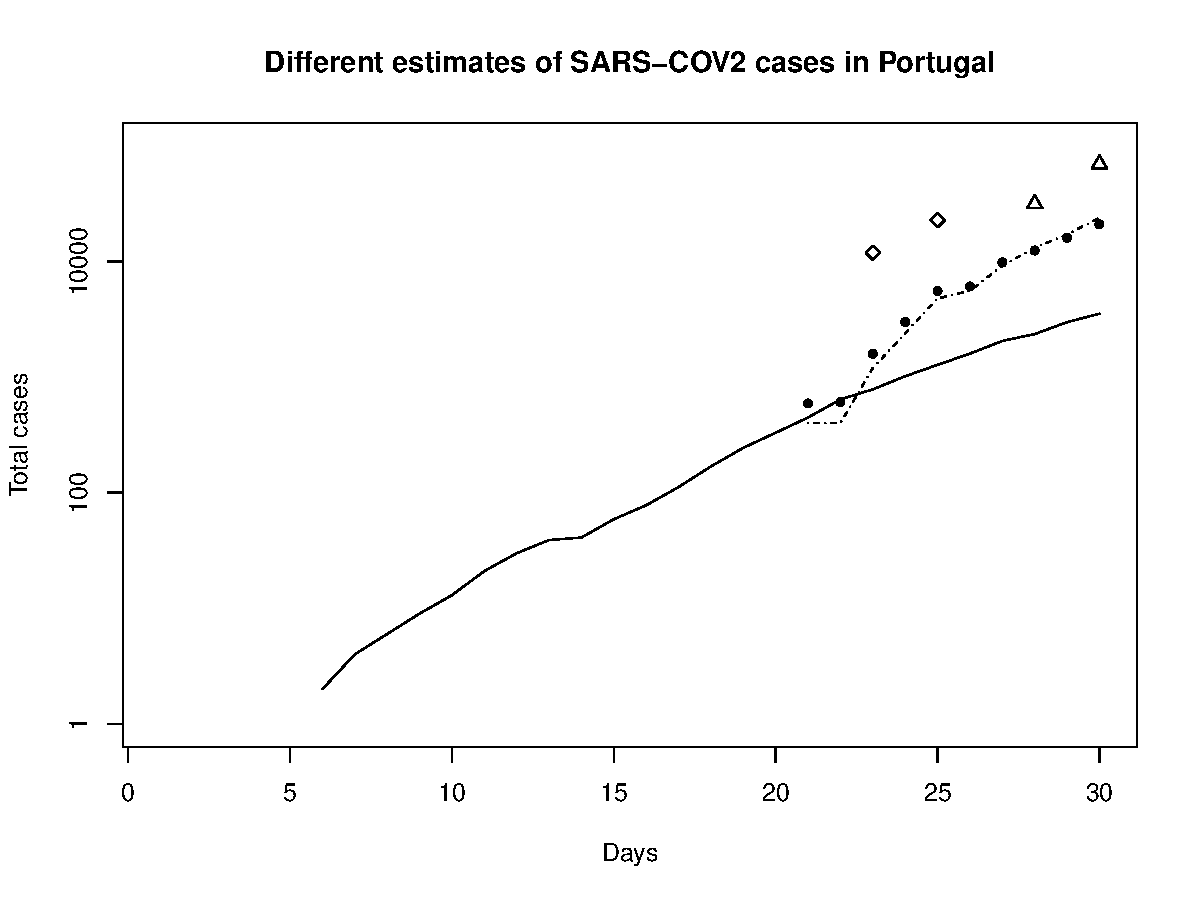
\includegraphics[width=.8\linewidth]{EstPTMar26.pdf}
\end{center}
\end{figure}

\section{The Spanish data}


\end{document}
